%!TeX program = xelatex
%Do not change
\documentclass[12pt, oneside]{article}
\usepackage{amssymb,amsmath}
\usepackage[margin=1in]{geometry}
\usepackage{textpos}
\usepackage{float}
\usepackage{booktabs}
%\usepackage{color}
\usepackage{graphicx}
\usepackage[inter-unit-product =\cdot]{siunitx}
\let\DeclareUSUnit\DeclareSIUnit
\let\US\SI
\DeclareUSUnit\inch{in}
\DeclareUSUnit\foot{ft}
\DeclareUSUnit\mile{mi}
\DeclareUSUnit\foot{ft}
\DeclareUSUnit\slug{slug}
\DeclareUSUnit\pound{lb}
\DeclareUSUnit\psi{psi}
\DeclareUSUnit\Msi{Msi}
\DeclareUSUnit\ksi{ksi}

%\usepackage{tikz}
%\usetikzlibrary{positioning}
%\usepackage{tikz-3dplot}
%\usepackage{pgfopts}
%\usepackage{wasysym}
%\usepackage{stanli}

% You may add the packages you need here
\begin{document}

%TODO change numbers in problems
\begin{textblock*}{4cm}(-1.7cm,-2.3cm)
\noindent {\scriptsize AE333 Fall 2020}
\end{textblock*}

%Do not modify other than putting your name where stated
\begin{textblock*}{8cm}(12.5cm,-1cm)
\noindent {Name: }
\end{textblock*}
%Do not modify other than typing your acknowledgement where stated
\begin{textblock*}{13.5cm}(-1.7cm,-1.8cm)
%\noindent \textit{\footnotesize Acknowledgement: Your acknowledgement for collaboration and other sources goes here. }
\end{textblock*}

\vspace{1cm}

%Do not modify other than typing the homework number after #
\begin{center}
\textbf{\Large Homework 7 Solutions}

\textbf{Due 27 October 2020}
\end{center}

\begin{enumerate}
	\item %8-6
		Find the maximum force, $P$, that can be exerted on the pistons such that the hoop stress in the cylinder does not exceed $\SI{3}{MPa}$.
		Each piston has a radius of $\SI{46}{mm}$ and the cylinder has a wall thickness of $\SI{1 }{mm}$
		\begin{figure}[H]
			\centering
			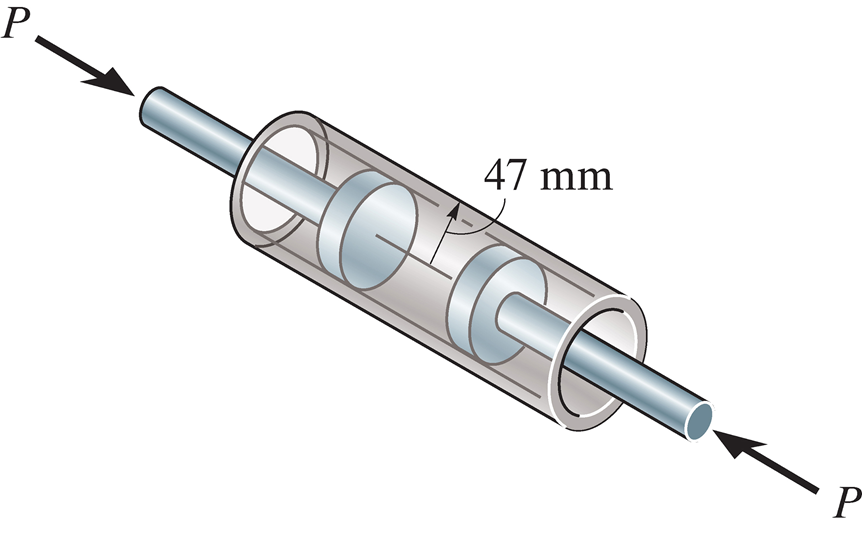
\includegraphics[width=0.6\linewidth]{8-6}
		\end{figure}
			\textbf{Solution:}
			\begin{itemize}
				\item The hoop stress is given as $\sigma_H = \frac{pr}{t}$ while the pressure is related to the applied force by $p = \frac{P}{\pi r^2}$
				\item Combining these gives hoop stress in terms of applied force $\sigma_H = \frac{Pr}{\pi r^2 t}$
				\item Solving for $P$ and substituting known values gives $P = 	\SI{434}{N} $
			\end{itemize}

	\item %8-9
		The steel water pipe has an inner diameter of $ 	\US{10}{in}  $ and a wall thickness of $ 	\US{.125}{in}  $.
		If the valve at $A$ is closed, find the stresses in the pipe at point $B$ when the water pressure is $ 	\US{250}{psi}  $.
		Sketch the state of stress on a representative element at $B$.
		\begin{figure}[H]
			\centering
			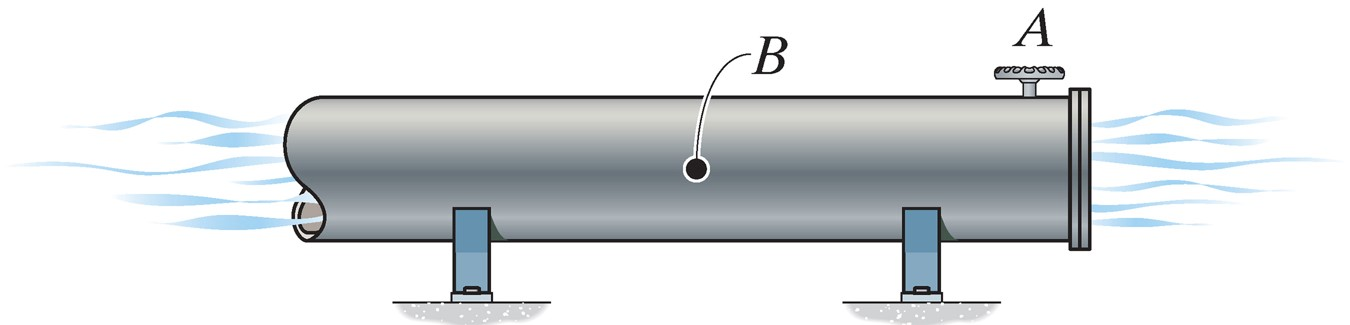
\includegraphics[width=0.6\linewidth]{8-9}
		\end{figure}
			\textbf{Solution:}
			\begin{itemize}
				\item When the pipe is open there will be no longitudinal stress, but when it closes the pipe will have both hoop and longitudinal stress.
				\item Hoop stress is $\sigma_H = \frac{p r}{t} = \frac{250(5)}{0.125} = 	\US{10}{ksi} $
				\item Longitudinal stress is $\sigma_L = \frac{p r}{2t} = \frac{250(5)}{2(.125)} = 	\US{5 }{ksi} $
					\begin{figure}[H]
						\centering
						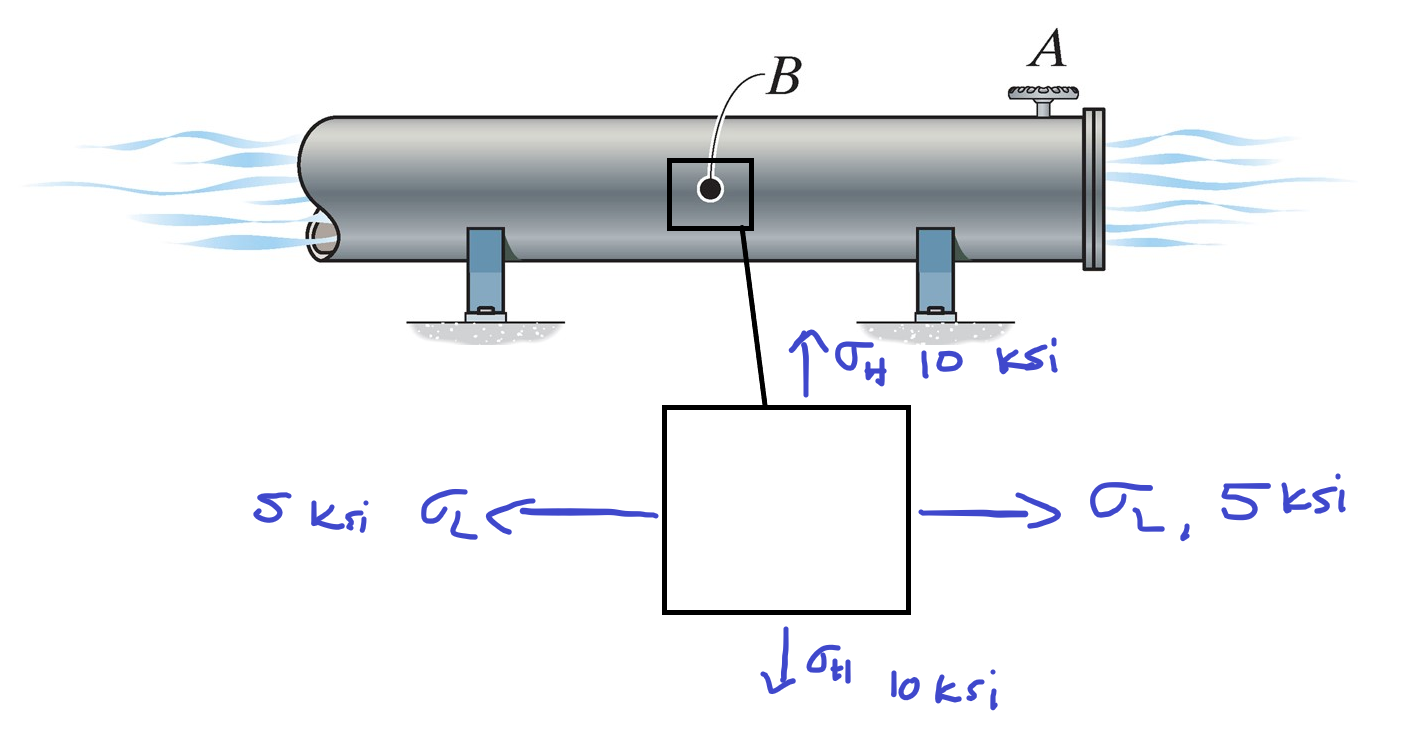
\includegraphics[width=0.6\linewidth]{8-9-ans}
					\end{figure}
			\end{itemize}

	\item %8-27
		The screw of a C-clamp exerts a compressive force of $ 	\US{500}{lb}  $ on the wood blocks.
		Sketch the stress distribution on section $a-a$ of the clamp assuming it has a rectangular cross section of $ 	\US{0.75}{in}  $ tall by $ 	\US{0.25 }{in }  $ thick.
		\begin{figure}[H]
			\centering
			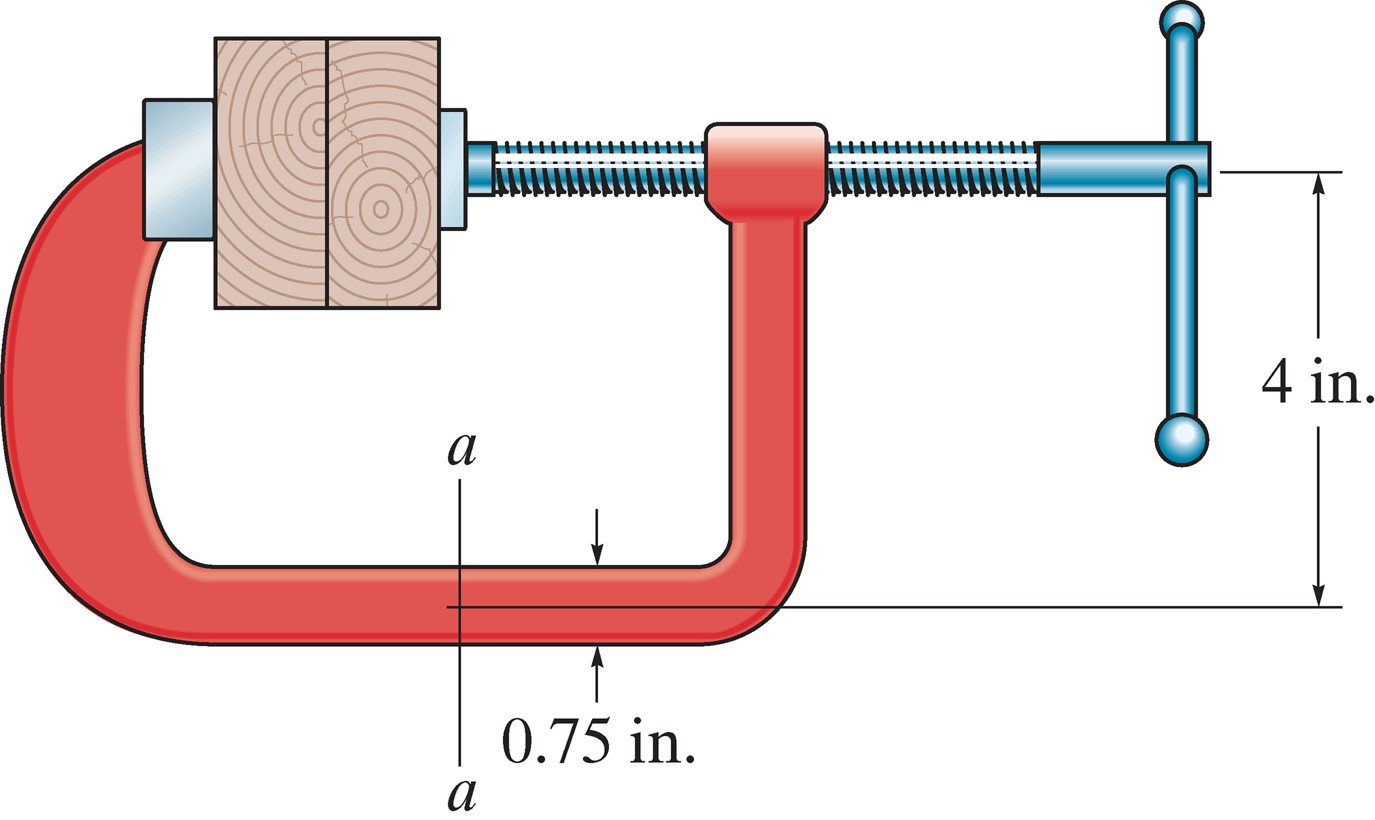
\includegraphics[width=0.6\linewidth]{8-27}
		\end{figure}
			\textbf{Solution:}
			\begin{itemize}
				\item When we section out the wood blocks, the reaction from the wood blocks pushes back against the c-clamp.
					Considering a section at $a-a$, we see that there is both an internal normal force, $N$ and moment, $M$, but no transverse shear, $V$ or any out-of-plane forces or moments.
			\item The normal stress is $\sigma = N/A = 500/(.75 \cdot .25) = 	\US{2.67}{ksi} $
			\item The bending stress is $\sigma = -My/I = -2000 y / (1/12 .25 (.75^3)) = 	\US[number-math-rm = \mathnormal, parse-numbers = false]{-228 y }{ksi} $
			\item These stresses will add together, so we can sketch the stress through the thickness as shown
				\begin{figure}[H]
					\centering
					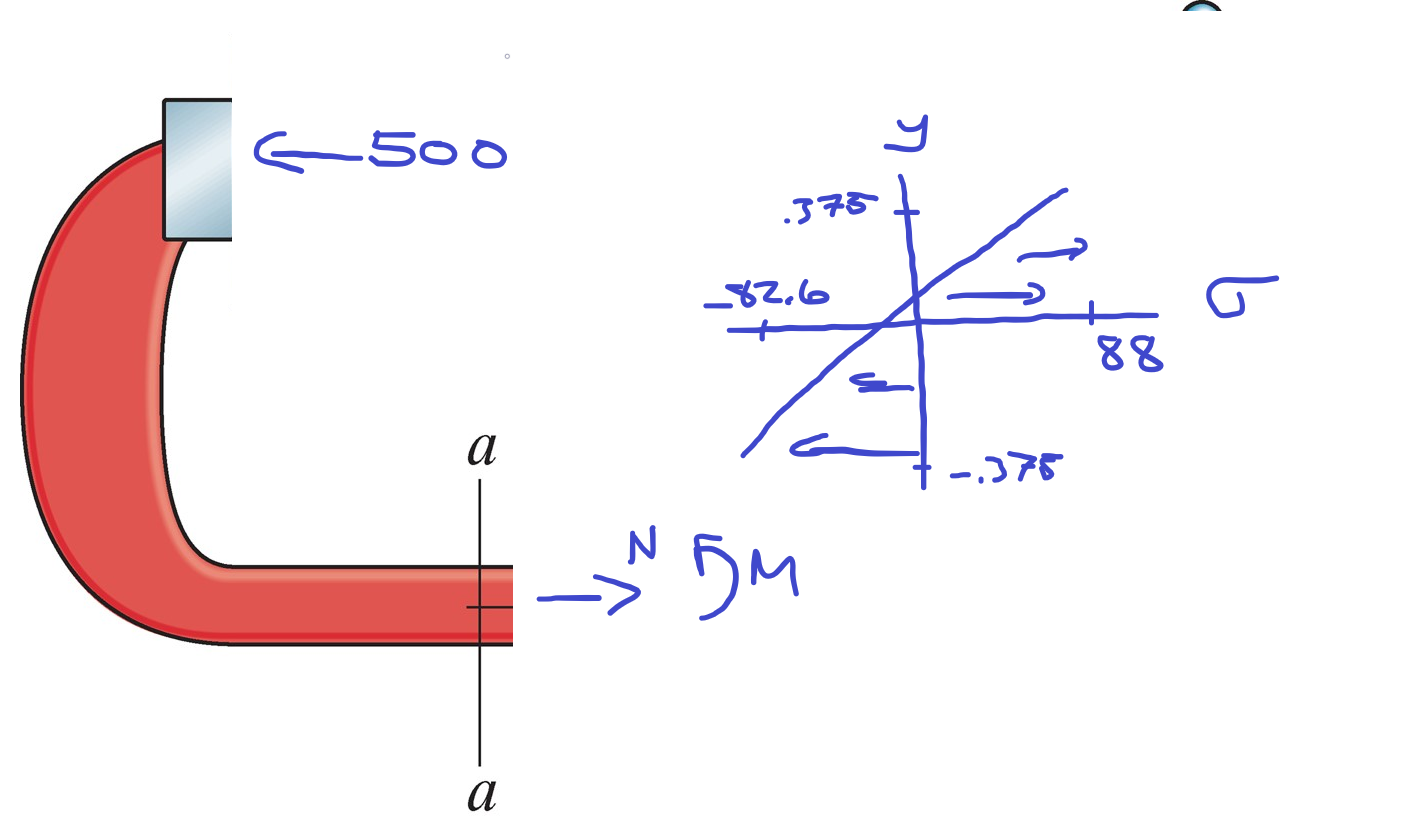
\includegraphics[width=0.6\linewidth]{8-27-ans}
				\end{figure}

			\end{itemize}

	\item %8-52
		The vertebra of the spinal column can support a maximum compressive stress of $\sigma_{max}$ before fracture.
		Find the smallest force, $P$, that would cause fracture if it is applied some distance $e$ away from the centerline of the bone.
		Treat the vertebra as a hollow cylinder.
		\begin{figure}[H]
			\centering
			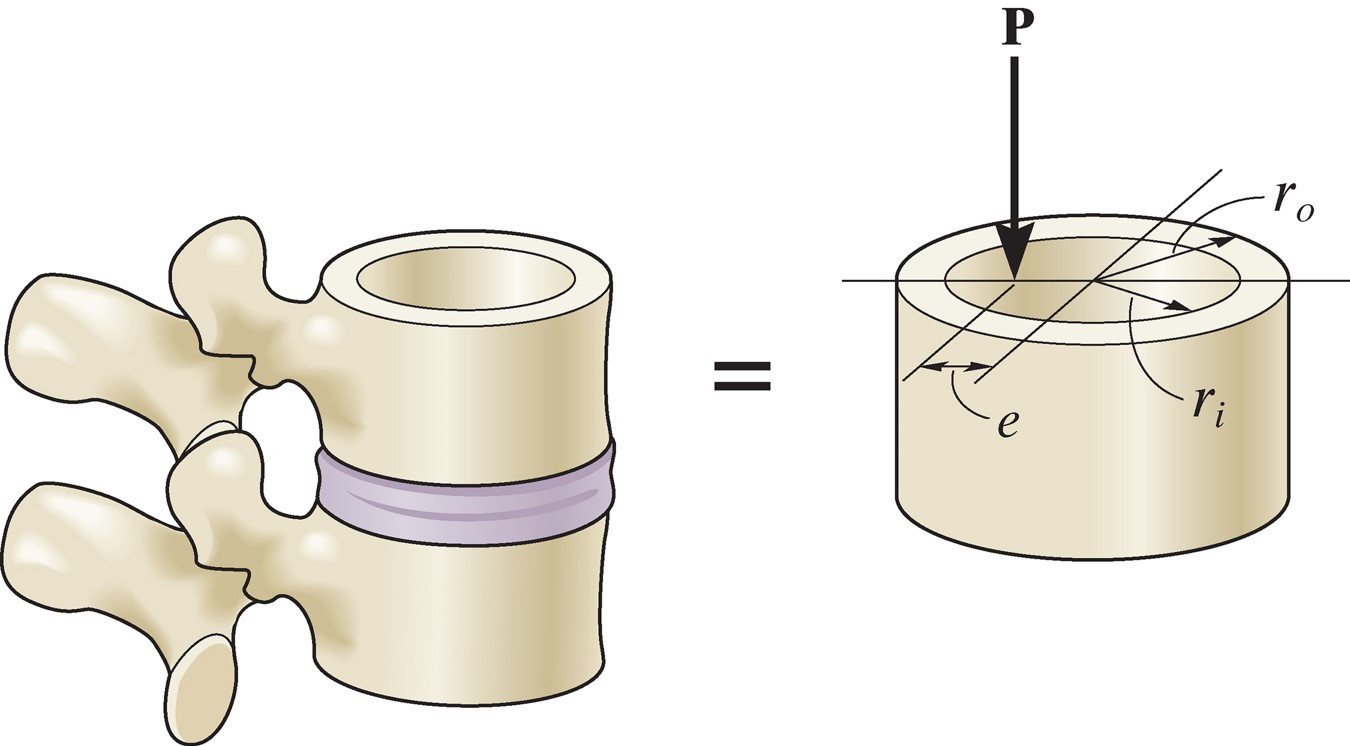
\includegraphics[width=0.6\linewidth]{8-52}
		\end{figure}
			\textbf{Solution:}
			\begin{itemize}
				\item The total compressive stress will be the sum of the normal compressive stress and bending, with the maximum bending occurring when $y=r_o$, this means we will have something like $\sigma = P/A + M r_o / I$ and we need to find $P$ in terms of other quantities
				\item From moment equilibrium, we find $M = Pe$, and substituting other known quantities we have $\sigma = \frac{P}{\pi(r_o^2-r_i^2)} + \frac{P e r_o}{\pi/4(r_o^4-r_i^4)}$
				\item We can factor out $P$, $\pi$ to find $\sigma = P \pi \left( \frac{1}{r_o^2 - r_i^2} \frac{4er_o}{r_o^4-r_i^4} \right)$ and finding a least common denominator and solving for $P$ gives $P = \frac{\sigma}{\pi}\left( \frac{r_o^4 - r_i^4}{r_o^2 + r_i^2 + 4er_o} \right)$
			\end{itemize}

	\item %past exam problem?
		Find the state of stress at the point $C$ indicated on the figure.
		\begin{figure}[H]
			\centering
			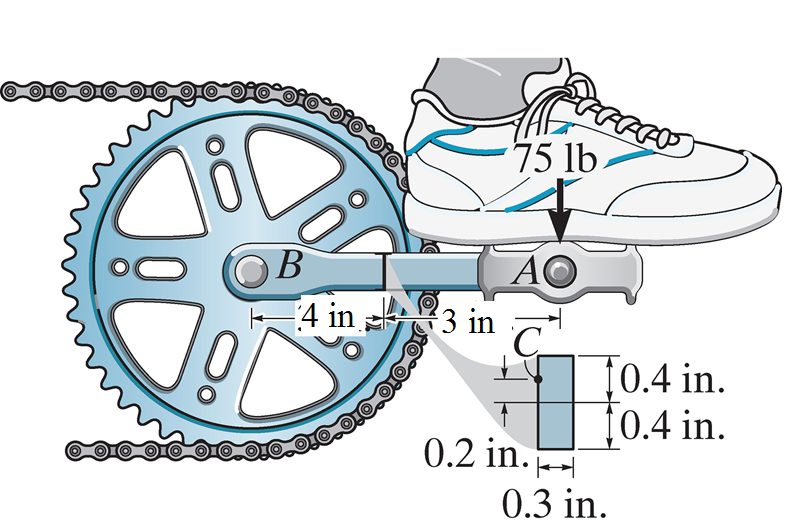
\includegraphics[width=0.6\linewidth]{3-2b}
		\end{figure}
			\textbf{Solution:}
			\begin{itemize}
				\item Sectioning to find the internal forces acting at the section where $C$ is we find that $N = 0$, $V = \US{75}{lb}$ and $M = \US{225}{in.lb}$.
				\item We can see from this stress state that we need to find the bending stress and the transverse shear stress
				\item Terms we will need in these calculations are $y = \US{0.2}{in}$, $I = \US{.0128}{in^4}$, $Q = \US{0.018}{in^3}$
				\item This gives $\sigma = \frac{My}{I} = \US{3.52}{ksi}$ and $\tau = \frac{VQ}{IT} = \US{352}{psi}$
			\end{itemize}

	\item %C8-1
		Explain why this garden hose failed along its length instead of in some other way.
		\begin{figure}[H]
			\centering
			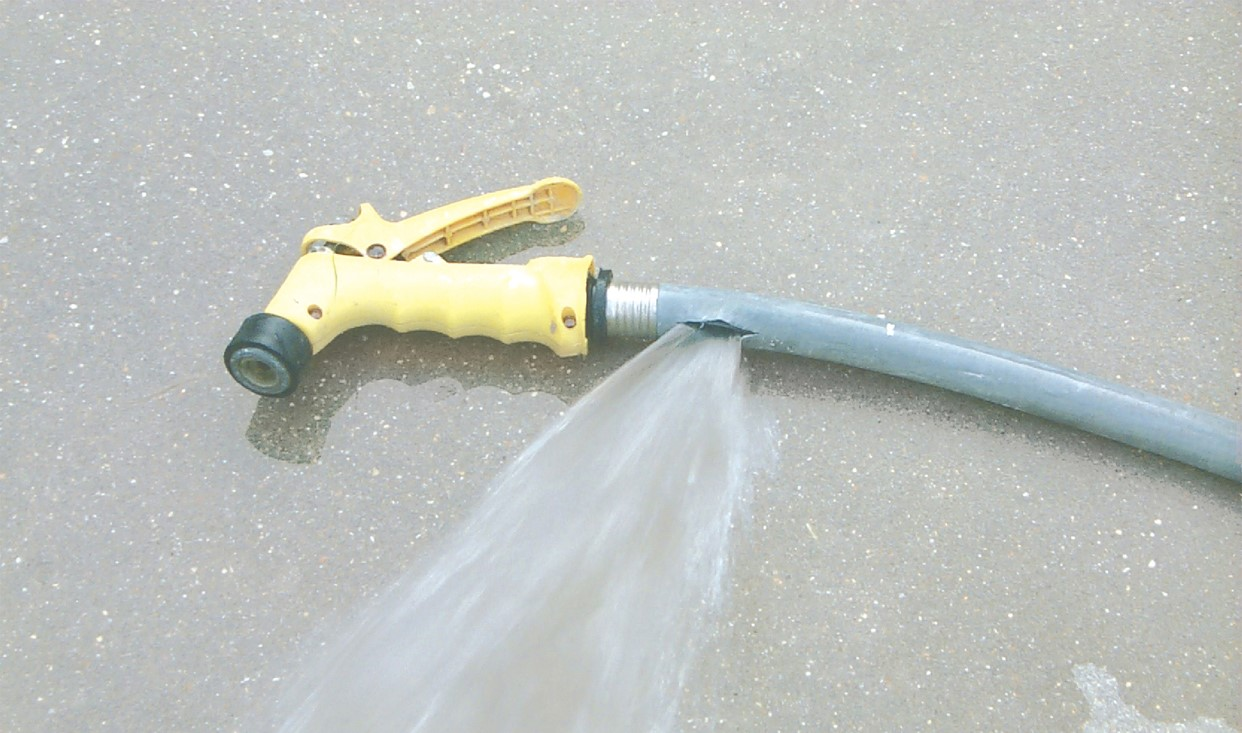
\includegraphics[width=0.6\linewidth]{C8-1}
		\end{figure}
			\textbf{Solution:}
			\begin{itemize}
				\item When water flows into the hose the entire hose is under pressure. 
					When the end is stopped, there will be both longitudinal and hoop stress.
					In a cylindrical vessel, the hoop stress will be double the longitudinal stress, which would cause the hose to split along its length the way that it has.
			\end{itemize}

	\item %C8-2
		This open-ended grain silo is used to store wheat or other grain.
		It is built from vertically-oriented wooden slates with steel straps holding them together.
		Explain why the bands are spaced closer together near the bottom compared to the top.
		If each band were to have the same stress, how would you determine the spacing?
		How is this silo different from a thin-walled pressure vessel?
		\begin{figure}[H]
			\centering
			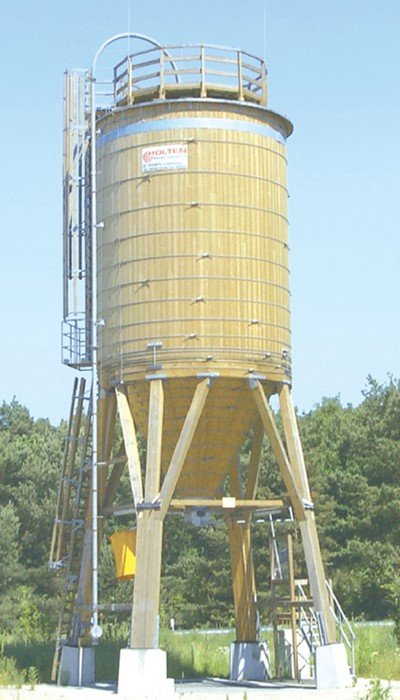
\includegraphics[width=0.6\linewidth]{C8-2}
		\end{figure}
			\textbf{Solution:}
			\begin{itemize}
				\item We can relate this silo to a pressure vessel, except with one end open there will be no longitudinal stress, only hoop stress and the pressure exerted on the sides will vary with height, instead of being constant.
				\item If we consider a slice of the silo, it will look similar to when we derived the hoop stress for a pressure vessel.
					One difference in this case is that the pressure will not be constant, but will instead vary with height.
					Since we have not established dimensions for the band, but we know that each steel strap will be the same we can say that the force in a band is equal to the force caused by the pressure over the region until the next band is reached, if we call that spacing $s$ and use $p = \rho g z$ then we find $\rho g z (s) (2r) = F$.
					Solving for the spacing, $s$ we find that $s = \frac{F}{2 \rho g z r}$
			\end{itemize}

\end{enumerate}
\end{document}
